%\textit{All code for simulation can be accessed from GitHub through this link:}

The entire model and simulation code can be found at \url{https://github.com/kiatvonj/dynein_walk}, where the model and simulation were coded using both Python and C++. The both bound Monte Carlo was coded on Python due to the calculations being less computationally rigorous and time independent, while the one bound Brownian dynamics was coded on C++ to utilize the faster computation speed for the time  dependent Brownian motion.

\section{Simulation}
%\textit{Picking Random angles to create random distribution of dynein configurations. Make sure to clarify that the simulation is split into two parts, the monte carlo both bound and brownian one bound. It is done this way in order for MC to generate ensemble of data rather quickly.}\\
%\textit{Include a flow chart.}
To generate an ensemble of steps, we use the Monte Carlo method to simulate a single step at a time, as opposed to a walk. This simplifies the code into two parts (the Monte Carlo both bound and the Brownian dynamics one bound) that cycle repeatedly after the model takes a step. The simulation starts in the both bound state, where the Monte Carlo randomly picks a both bound configuration and calculates the total energy. If the configuration successfully unbinds, then we use the positions of the domains as initial conditions for the one bound simulation and execute the Brownian dynamics. Once the one bound dynein diffuses onto the microtubule and rebinds, the simulation repeats the cycle and generates a completely different both bound configuration for another step. However, this method comes with a caveat: we must initialize the distance between the binding domains, $L$, to ensure that our ensemble covers the whole sample space of possible both bound configurations. This forces the measured probabilities to be a function of $L$ and will be addressed later in the Data Analysis section (Section \ref{sec:DataAna}). The algorithm for the both bound process is shown below:

\newpage
\begin{center}\label{alg:MonteCarlo}
	\textbf{\underline{Monte Carlo Algorithm}}
\end{center}


\begin{enumerate}
	\item Initialize an unsigned distance, $L$, between the binding domains.
	
	\item Randomly pick 4 angles ($\theta_0$, $\theta_1$, $\theta_2$, $\theta_3$) to generate a completely random configuration of dynein in space.
	
	\item Calculate the distance between the binding domains and check if the distance is within a range of $L\pm l$, where $l$ is arbitrarily small.
	   \davidsays{Mention going back to 2 if the distance isn't in range.}
\end{enumerate}

\begin{figure}[H]
\centering
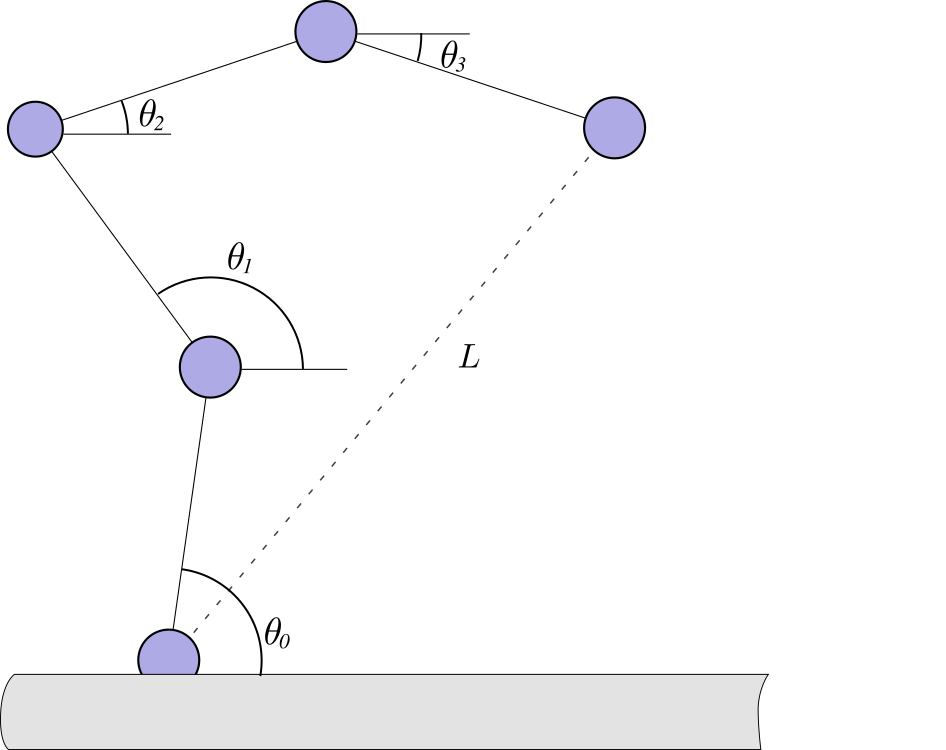
\includegraphics[width=0.5\columnwidth]{Figures/montecarlo2.png}
%\caption[Dynein Model]{\textbf{Dynein Model.} }
\label{fig:mc2}
\end{figure}

\begin{enumerate}
	\setcounter{enumi}{3}
	\item Rotate the configuration so that both binding domains are on the microtubule and recalculate angles with the naming convention in Figure (\ref{fig:OBvsBB}).
\end{enumerate}

\begin{figure}[H]
\centering
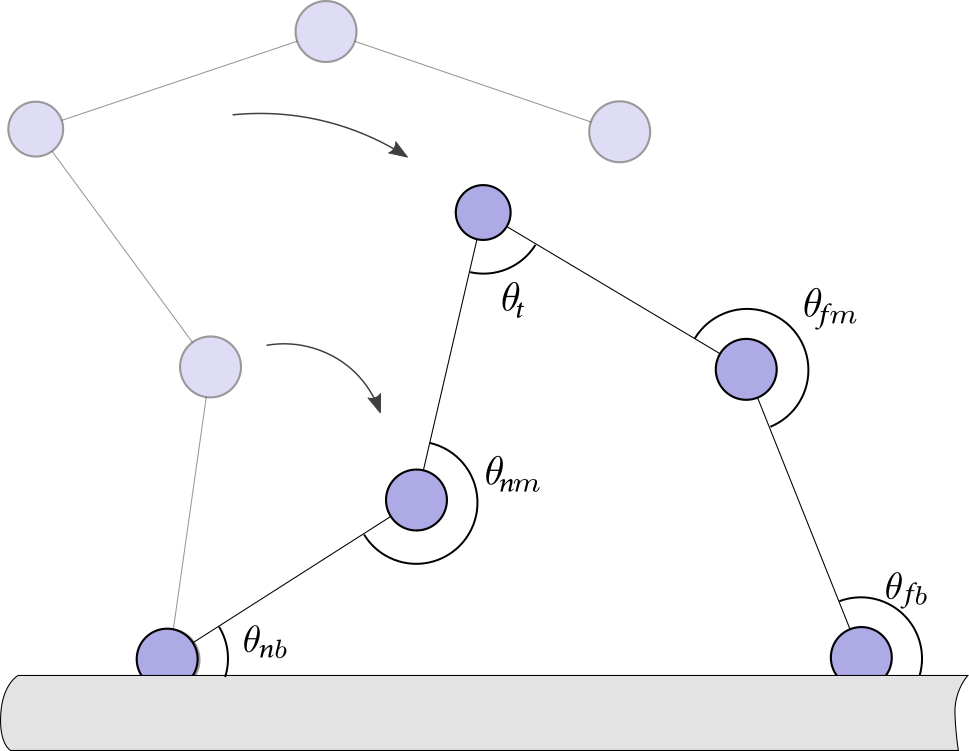
\includegraphics[width=0.5\columnwidth]{Figures/montecarlo3.png}
%\caption[Dynein Model]{\textbf{Dynein Model.} }
\label{fig:mc3}
\end{figure}

\begin{enumerate}
	\setcounter{enumi}{4}
	\item Calculate the total energy of the configuration by summing the energy of each domain (using Equation (\ref{eqn:energy})) and the relative unbinding probability from a Boltzmann distribution,
	\begin{equation}
		E_{total, i}=\sum_{k}\frac{1}{2}c_k(\theta_k-\theta_{k,eq})^2,
	\end{equation}
	\begin{equation}
		P_{ub} \propto \rho_{ub}e^{-\beta E_{total, i}}\kappa.
	\end{equation}
	Then, add a term to the partition function,
	\begin{equation}
		Z=\sum_{i}e^{\beta E_{total, i}}.
	\end{equation}
	Here, $i$ refers to the specific both bound configuration and $k$ is the domain. We also defined $\kappa$ to normalize the relative unbinding probability to keep it less than 1. 
	
	\item ``Roll a die" for a value within the range of $[0,1]$ and check if the value is less than $P_{ub}$. If not, repeat algorithm from step 2.
\end{enumerate}

\begin{figure}[H]
\centering
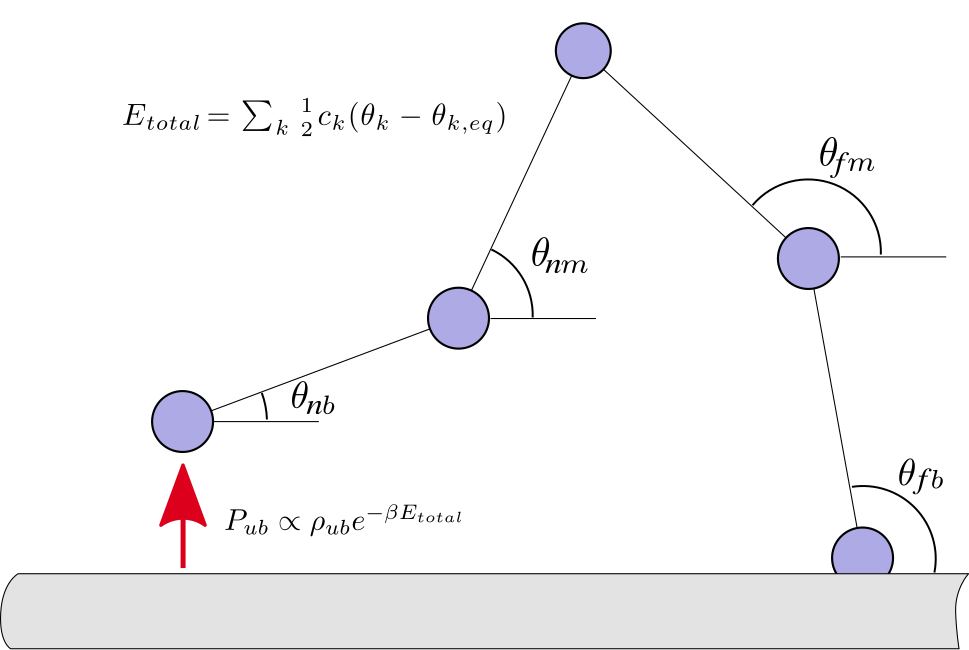
\includegraphics[width=0.8\columnwidth]{Figures/montecarlo4.png}
%\caption[Dynein Model]{\textbf{Dynein Model.} }
\label{fig:mc4}
\end{figure}

\newpage

\begin{enumerate}
	\setcounter{enumi}{6}
	\item If dynein unbinds, initialize the one bound state with the both bound configuration, run the Brownian dynamics simulation of the step, and wait until it rebinds.
\end{enumerate}

\begin{figure}[H]
\centering
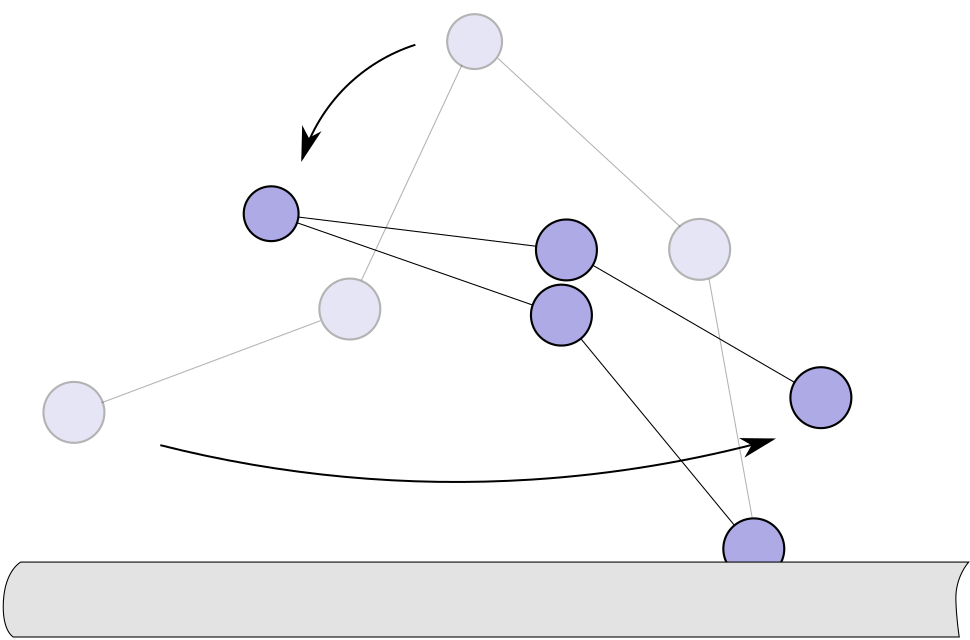
\includegraphics[width=0.7\columnwidth]{Figures/montecarlo5.png}
%\caption[Dynein Model]{\textbf{Dynein Model.} }
\label{fig:mc4}
\end{figure}

\begin{enumerate}
	\setcounter{enumi}{7}
	\item Collect statistics about the final position and one bound time. Repeat algorithm from step 2. 
\end{enumerate}

\begin{figure}[H]
\centering
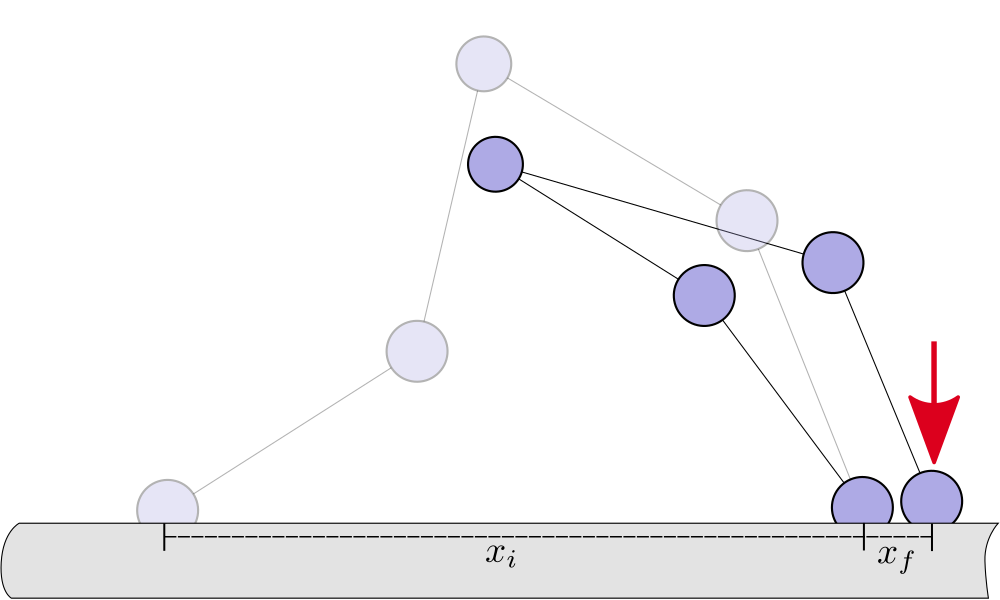
\includegraphics[width=0.7\columnwidth]{Figures/montecarlo6.png}
%\caption[Dynein Model]{\textbf{Dynein Model.} }
\label{fig:mc4}
\end{figure}

\noindent\rule{16.5cm}{0.4pt}

A more in-depth explanation and rigorous flow chart for the one bound Brownian dynamics simulation can be found here \cite{Capek2017, }.


%\section{Time Evolution}
%\textit{Simulate over a delta t during one bound and every iteration check for rebinding. How are the probabilities of binding and unbinding affected by the time.}

\section{Model Parameters}
%\textit{How we defined our constants based on experiment and pictures.  Need to include figures here of experiment dynein and how we measure the pre and post stroke equilibrium angles.}

We match model paramters concerning dynein's geometry based on experiment by analyzing electron microscopy pictures of dynein. These pictures are shown in Figure (\ref{fig:ParamsPics}), where experimental dynein is in the conformations analogous to the both bound and one bound states. We can measure the domain radii \{$R_i$\}, equilibrium angles \{$\theta_{i,eq}$\}, and the stalk and tail lengths ($L_s$, $L_t$) from these figures (refer to Section \ref{sec:Params} for measurements).  

\begin{figure}[hbt!]
	\centering
	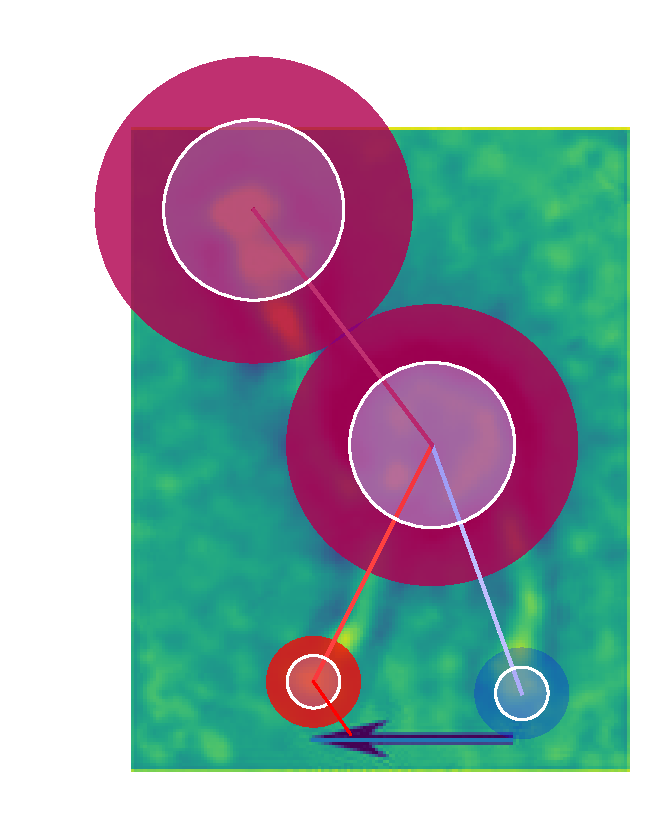
\includegraphics[width=0.3\columnwidth]{../../plots/burgess-model-figure.pdf}
	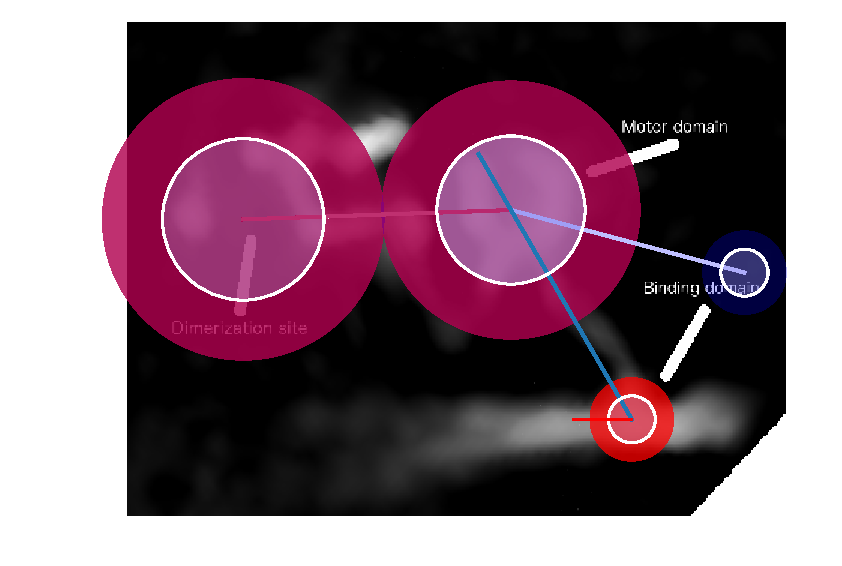
\includegraphics[width=0.5\columnwidth]{../../plots/grotjahn-model-figure.pdf}%
	\caption[Experimental Pictures of Dynein for Model Parameters]{\textbf{Experimental Pictures of Dynein for Model Parameters} \textit{Left:} Micrograph of both bound dynein with model domains to identify post-stroke equilbrium angles. The arrow indicates 15 nm \cite{Burgess2003}.  \textit{Right:} Cryo-electron tomograph of one bound dynein for pre-stroke equilbrium angles \cite{grotjahn2018cryo}.} 
	\label{fig:ParamsPics}
\end{figure}

However, these pictures do not help identify the binding rates ($k_a$, $k_b$, $k_{ub}$) and spring constants ($c_b$, $c_m$, $c_t$), making these parameters \textit{free variables} in the model. Fortunately, the Monte Carlo simulation can quickly optimize these free variables and fit different combinations of parameters to  different sets of experimental data. Since we want to replicate Yildiz's observations from Figure (\ref{fig:YildizCorrelation}), the free variables will be optimized according to the slope and y-intercept of the correlation. 

\subsection{Validation for Model Parameters}
%\textit{Fitting our rate constants were a huge part of our model and how we made sure our dynein can match experimentalist results. Maybe bring up sticky rate???}

Despite simulating many combinations of parameters, the number of free variables still produce many degrees of freedom. This makes it difficult to test the entire parameter space and truly invesitage the relationships between different sets of parameters. We approach this problem by individually attributing the parameters to a specific data set from exerpiment. For instance, the exponential unbinding constant, $C$, is fitted specifically to Figure (\ref{fig:trailingbias}). We use time data (\textit{cite paper for time data}\cite{}) to fit the unbinding rate constant, $k_{ub}$, because the inverse yields the average time it takes to unbind, i.e. the both bound time. The rebinding rates, $k_a$ and $k_b$, are harder to optimize because they directly correlate to step length. The ability for dynein to take long steps is dependent on how long dynein diffuses above the microtubule. Therefore, the rebinding rates have a much larger parameter space due to the flexibility of optimizing according to the one bound time or step length. Since we are interested in Yildiz's step lengths, we match these rates to the linear regression from Figure (\ref{fig:YildizCorrelation}) and Yildiz's step length plots. The last parameters are the spring constants. The spring constants also influence the step length because they dictate the strength of the restoring force. We fit the spring constants last to control the variance of step lengths.


%An increase in the binding rate will cause fast steps and significantly shorter step lengths that approach 0nm (rebinds where foot unbinded). This causes a dilemma because experiments cannot record step lengths close to 0nm. 


\section{Data Analysis} \label{sec:DataAna}
As mentioned earlier, the simulation collects statistics only for a given initial binding domain distance, $L$. This limits the probability data of landing at a final position to be a function of $L$. However, we can not calculate the step length for a trailing or leading step with an unsigned distance. This promotes the new naming scheme of using initial and final displacement, $x_i$ and $x_f$, when identifying the distances between the binding domains before and after the step. The displacement is the $x$ position of the unbounded binding domain, where the origin is defined at the bounded binding domain. This implies a negative initial displacement for a trailing step and a positive initial displacement for a leading step. 

However, the simulation still outputs a probability distribution of final displacements as a function of initial displacements. To properly reproduce Yildiz's stepping plot, we need a joint probability distribution with both $x_i$ and $x_f$ as variables. Using probability notation, we want $p(x_i,x_f)$ (the probability of $x_i$ \textit{and} $x_f$) but we have $p(x_f|x_i)$ (the probability of $x_f$ \textit{given} $x_i$). To solve this problem, we can use conditional probability and solve for $p(x_i,x_f)$, as shown below:


\[
	p(x_f|x_i)=\frac{p(x_i,x_f)}{p(x_i)},
\]
\begin{equation}
	p(x_i,x_f)=p(x_f|x_i)p(x_i).
\end{equation}
Now, we only need to find the probability density of initial displacements, $p(x_i)$. Since the initial displacement is simply a signed distance $L$, we can use the probability of unbinding for a trailing or leading step as a function of $L$ from Equation (\ref{eqn:ProbTrail}) to generate $p(x_i)$. In other words, Equation (\ref{eqn:ProbTrail}) gives us $p(x_i|L_i)$. We can relate the two by using Bayes' Theorem,

\begin{equation}
	p(x_i|L_i)=\frac{p(L_i|x_i)p(x_i)}{p(L_i)}.
\end{equation}
Since the probability of an initial distance given the initial displacement, $p(L_i|x_i)$, is always 1, we can simplify further,
\[
	p(x_i|L_i)=\frac{p(x_i)}{p(L_i)},
\]

\begin{equation}
	p(x_i)=p(x_i|L_i)p(L_i).
\end{equation}
Now, the final step is to solve for the probability distribution of distances, $p(L_i)$. Since we want the probability of absolute differences, we can neglect the distinction between `initial' and `final' and calculate an equilibrium distribution of distances, $p(L)$. To do so, we use a reccurence relation, where we define an initial $p^0(L)$ that is not in equilibrium and multiply it by the conditional probability distribution for arbitrary $L$'s, $p(L'|L)$, until it reaches equilibrium. That is,
\begin{align*}
	p^1(L)= & p(L'|L)p^0(L) \\
	p^2(L)= & p(L'|L)p^1(L)=p(L'|L)^2p^0(L)\\
	&\vdots \\
	p^n(L)= & p(L'|L)p^{n-1}(L)=p(L'|L)^np^0(L) 
\end{align*}
\begin{equation}
	p^n(L)=p(L'|L)^np^0(L) 	
\end{equation}
where $n$ is an arbitrarily large number of steps to ensure the dynein is in equilibrium. This process can be thought of as a large row of dyneins all starting with the probability of an initial distance $p^0(L)$. Once they all take a step, their probability of having another distance $L'$ is $p(L'|L)p(L)$, and after a significant number of $n$ steps, the probability of having a distance $L$ would be the same for all the dyneins, thus being an equilibirum distribution of $L$. To solve for $p(L'|L)$, we can use the previous probability distributions $p(x_f|x_i)$ and $p(x_i|L_i)$ to convert these probabilities into distances, as shown below:
\begin{equation}
	p(L'|L)=I(L'|x_i)p(x_f|x_i)p(x_i|L),
\end{equation}
where $I(L'|x_i)$ is the identity matrix for converting $x_f$ into $L'$. We have now solved for all the unknowns to generate a joint probability distribution of initial and final displacements, $p(x_i,x_f)$. 


